\documentclass[tikz,border=2pt]{standalone}
\usepackage{amsmath,amssymb}
\usepackage{tikz}
\usetikzlibrary{arrows.meta}

\begin{document}
% A budget-type problem max f(x) s.t. x_1 + x_2 = s: as the parameter s changes the constraint
% line shifts, the optimum x*(s) moves along a path, and the optimal value V(s) changes.
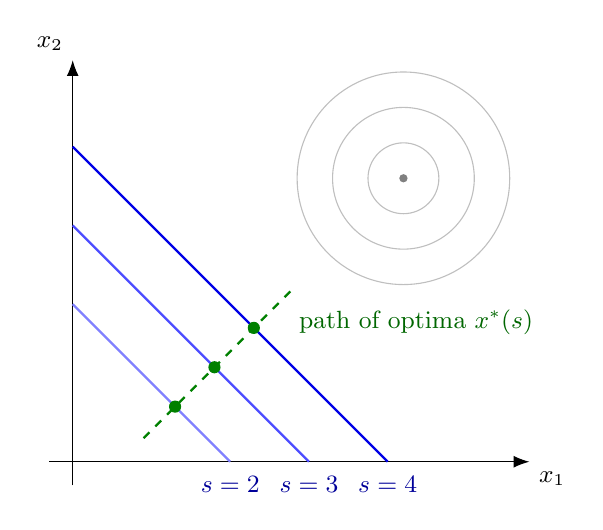
\begin{tikzpicture}[every node/.style={font=\small}, >={Latex[length=2mm]}]
	\foreach \r in {0.45,0.9,1.35} {\draw[gray!50] (4.2,3.6) circle (\r);}
	\fill[gray] (4.2,3.6) circle (1.5pt);
	\draw[->] (-0.3,0) -- (5.8,0) node[below right] {$x_1$};
	\draw[->] (0,-0.3) -- (0,5.1) node[above left] {$x_2$};
	\draw[blue!50, thick] (2,0) -- (0,2);
	\draw[blue!70, thick] (3,0) -- (0,3);
	\draw[blue!90!black, thick] (4,0) -- (0,4);
	\node[blue!60!black, font=\small, anchor=north] at (2,-0.06) {$s=2$};
	\node[blue!60!black, font=\small, anchor=north] at (3,-0.06) {$s=3$};
	\node[blue!60!black, font=\small, anchor=north] at (4,-0.06) {$s=4$};
	\draw[green!50!black, thick, dashed] (0.9,0.3) -- (2.8,2.2);
	\fill[green!50!black] (1.3,0.7) circle (2.2pt);
	\fill[green!50!black] (1.8,1.2) circle (2.2pt);
	\fill[green!50!black] (2.3,1.7) circle (2.2pt);
	\node[green!40!black, font=\small, anchor=north west] at (2.75,2.05) {path of optima $x^\ast(s)$};
\end{tikzpicture}
\end{document}
